\documentclass[12pt]{jarticle}

\usepackage[dvipdfmx]{graphicx}
\usepackage{url}
\usepackage{listings,jlisting}
\usepackage{ascmac}
\usepackage{amsmath,amssymb}
\usepackage{comment}

%ここからソースコードの表示に関する設定
\lstset{
  basicstyle={\ttfamily},
  identifierstyle={\small},
  commentstyle={\smallitshape},
  keywordstyle={\small\bfseries},
  ndkeywordstyle={\small},
  stringstyle={\small\ttfamily},
  frame={tb},
  breaklines=true,
  columns=[l]{fullflexible},
  numbers=left,
  xrightmargin=0zw,
  xleftmargin=3zw,
  numberstyle={\scriptsize},
  stepnumber=1,
  numbersep=1zw,
  lineskip=-0.5ex
}
%ここまでソースコードの表示に関する設定

\title{知能プログラミング演習II 課題6}
\author{グループ8\\
  29114142 湯浅範子\\
}
\date{2019年1月3日}

\begin{document}
\maketitle

\paragraph{提出物} rep6(2914142.pdf),group08.zip
\paragraph{グループ} グループ8
\paragraph{メンバー}
\begin{tabular}{|c|c|c|}
  \hline
  学生番号&氏名&貢献度比率\\
  \hline\hline
  29114003&青山周平&\\
  \hline
  29114060&後藤拓也&\\
  \hline
  29114116&増田大輝&\\
  \hline
  29114142&湯浅範子&\\
  \hline
  29119016&小中祐希&\\
  \hline
\end{tabular}

\section{課題の説明}
\begin{description}
\item[必須課題6-1] 課題5にやり残した発展課題があれば参考にして拡張しても良いし,全く新しい独自仕様を考案しても構わない.自由に拡張するか,あるいはもし残っていた問題点があれば完成度を高めよ.
\end{description}
私は前回課題の必須課題5-4のGUI実装の改良を行ったため,それについて記述する.

\section{必須課題6-1}
\begin{screen}
  課題5にやり残した発展課題があれば参考にして拡張しても良いし,全く新しい独自仕様を考案しても構わない.自由に拡張するか,あるいはもし残っていた問題点があれば完成度を高めよ.
\end{screen}
私の担当箇所は,前回課題で作成したGUIの改良である.

\subsection{手法}
前回のGUIに以下のような機能を加えた.

\begin{itemize}
\item ウィンドウサイズの変更時に起きたボタンのバグの解消
\item 動作を動的に表示

%\item 禁止制約変更操作
\end{itemize}

今回の改良では,前回の課題で時間の都合などで出来なかった部分の機能の拡張を行った.

\subsection{実装}
作成したGUIプログラムの中の改良部分についての実装を以下に示す.\\

まず,プランニングボタンをクリックして経路導出を行ったときの再描画時の動作をソースコード\ref{re}に示す.\\

\begin{lstlisting}[caption=再描画時の動作,label=re]
presenter.restart();
pUR = presenter.getStepList();
result = presenter.getPlan();
if (result != null) {
	results = new ArrayList<>(result);
	results.add(0, "default position");
} else {
	// 禁止制約に引っかかった時
	results = new ArrayList<>();
	results.add("default position");
}
page1.removeAll();
cardPanel.removeAll();
btnPanel.removeAll();
for (JPanel c : card) {
	c.removeAll();
}
createResultPage(pUR);
createButton();
finishData();
\end{lstlisting}

Presenterクラスのrestartメソッドを用い,変更した状態でプログラムを動作させる.得られた結果に応じて描画内容を変更するが,このときremoveAllメソッドを用いることで,現在あった描画内容を一度全て削除することが出来る.これを行わずとも再描画を行うことは可能であるが,その場合はマウスの動作に応じて出力が二重になって現れるなど誤作動が起きる場合がある.そのため,一度記述内容を削除してから再描画を行うことで誤作動を無くした.\\

次に,出力結果を動的に表示するためのプログラムをソースコード\ref{timer}に示す.\\

\begin{lstlisting}[caption=動的表示用,label=timer]
// 変数定義
Timer timer;
int time;
・・・
// タイマーの設定
timer = new Timer(1100 , this);
timer.setActionCommand("timer");

// 動的操作開始クラス(マウスクリックに対応)
public class myListener extends MouseAdapter{
	public void mousePressed(MouseEvent e){
		layout.show(cardPanel, "label0");
		time = 0;
		timer.start();
		firstButton.setEnabled(false);
		prevButton.setEnabled(false);
		nextButton.setEnabled(false);
		lastButton.setEnabled(false);
	}
}

// タイマーの動作設定
public void actionPerformed(ActionEvent e){
	// ボタン選択アクション
	String cmd = e.getActionCommand();
	・・・
	else if (cmd.equals("timer")){
		if (time < cardPage) {
			layout.next(cardPanel);
			time++;
		} else if (time == cardPage) {
			layout.next(cardPanel);
			firstButton.setEnabled(true);
			prevButton.setEnabled(true);
			nextButton.setEnabled(true);
			lastButton.setEnabled(true);
			timer.stop();
			time = 0;
		}
	}
}
\end{lstlisting}

前回の課題では,導出結果の結果を順に確認するためにはユーザーが毎回Nextボタンをクリックする必要があった.この方法でも結果の確認を行えるが,一連の動作を流れで確認したい時には手間がかかる.そのため今回の改良ではMoveボタンを新たに作成し,ユーザーがMoveボタンを一度クリックしただけで導出結果を順に全て確認できるようにした.\\

改良にあたり,タイマークラスを利用した.Moveボタンをクリックするとタイマーが動作を開始し,一定秒数ごとに経路を順に表示する.この動作中に他のボタンをクリックすると正しい動作が得られなくなってしまうため,経路の動的表示を行っている間は他のボタンを無効にすることで対処した.

\subsection{実行例}
初めに,ウィンドウサイズの変更時に起きたボタンのバグの解消結果を示す.\\
%\clearpage
まず,ウィンドウサイズを変更した際に起きるバグは以下の画像から分かる(図\ref{fig:ButErr}).これはウィンドウ作成時には起きず,再描画後に表示されるウィンドウサイズをユーザーが変更した際に起きる.\\

\begin{figure}[htbp]
  \begin{center}
    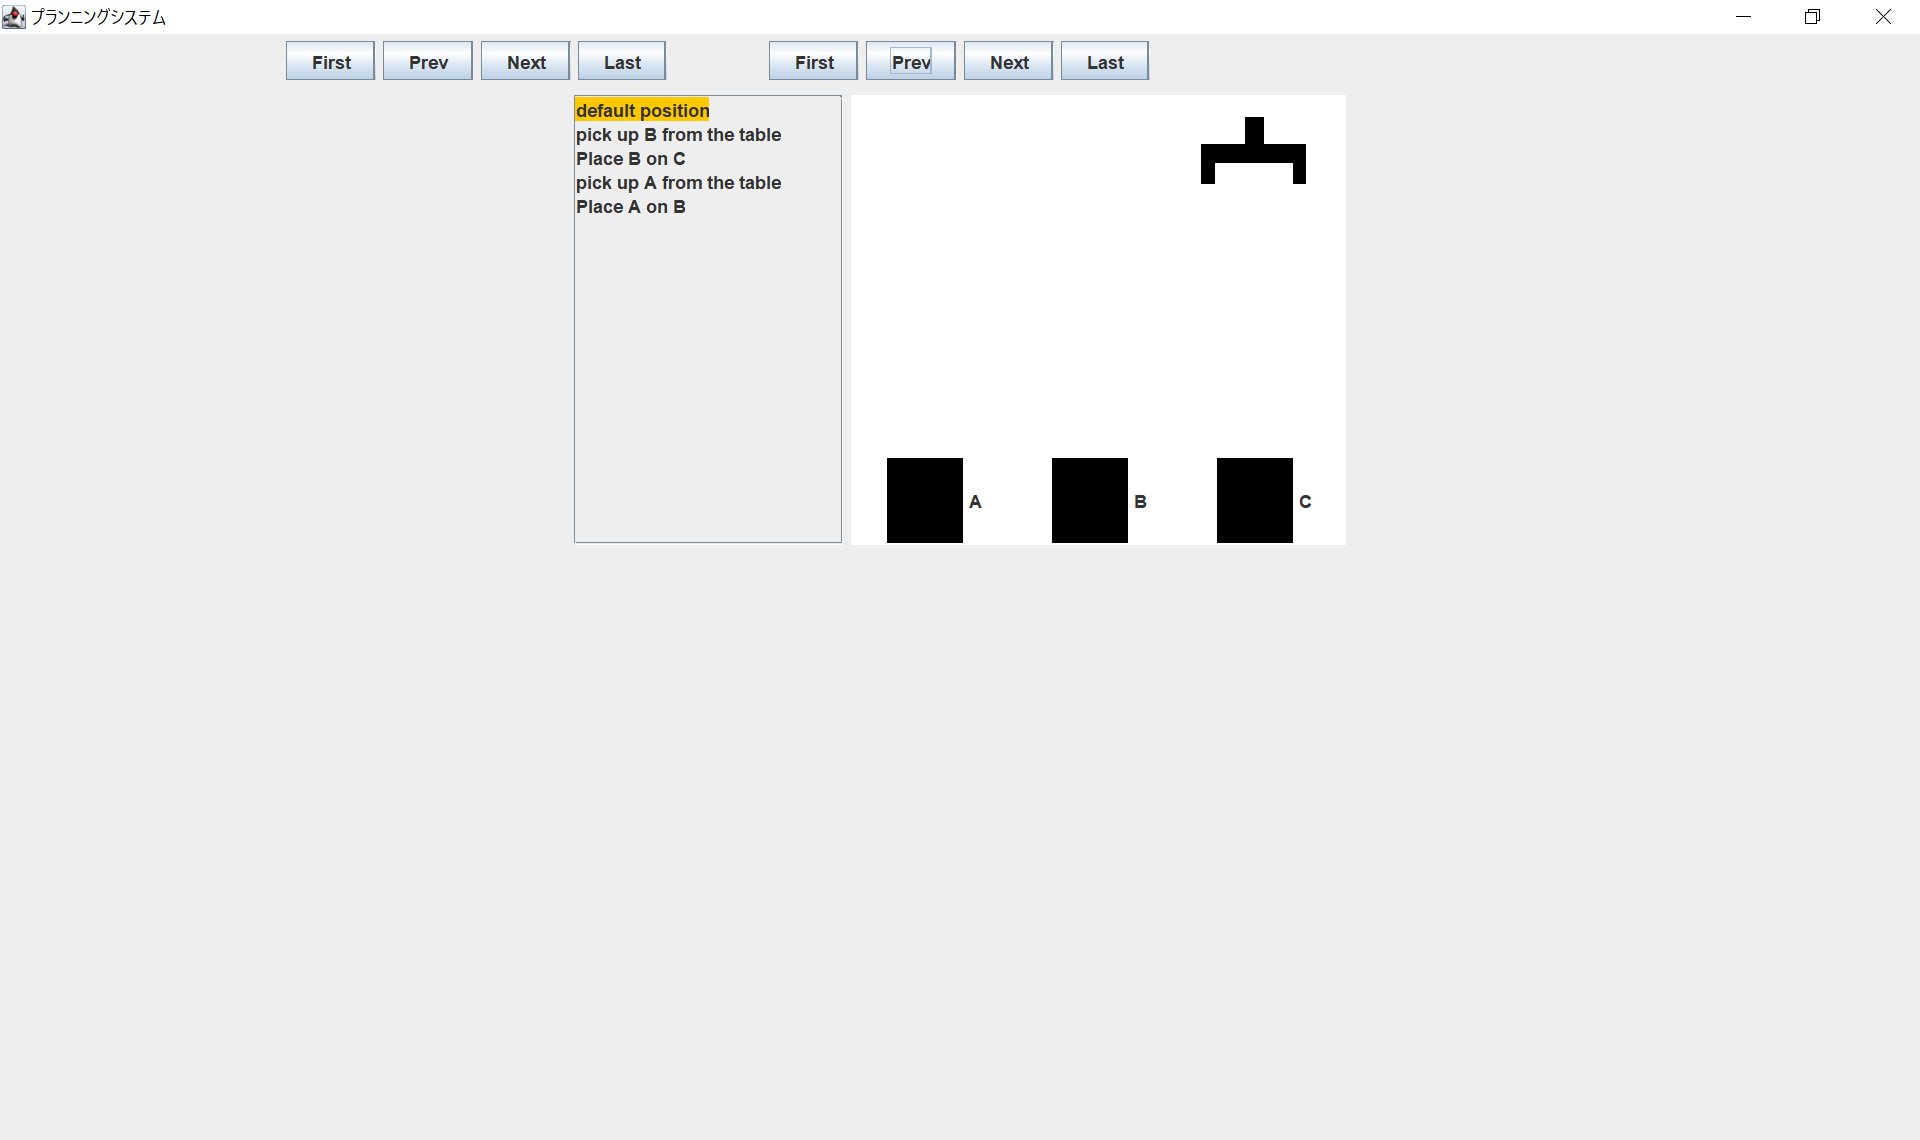
\includegraphics[scale=0.4]{images/ButErr.PNG}
    \caption{ウィンドウサイズを変更した際に起きるバグ}
    \label{fig:ButErr}
  \end{center}
\end{figure}
画像からも分かるように上に表示されるボタンの数が二重に表示されている.このときどちらのボタンも正しく動作を行うが,ウィンドウサイズの大きさによってはボタンが重なって表示されてしまうこともある.\\

\clearpage

これを改良した後の状態が,以下のようになる(図\ref{fig:ButOK}).\\

\begin{figure}[htbp]
  \begin{center}
    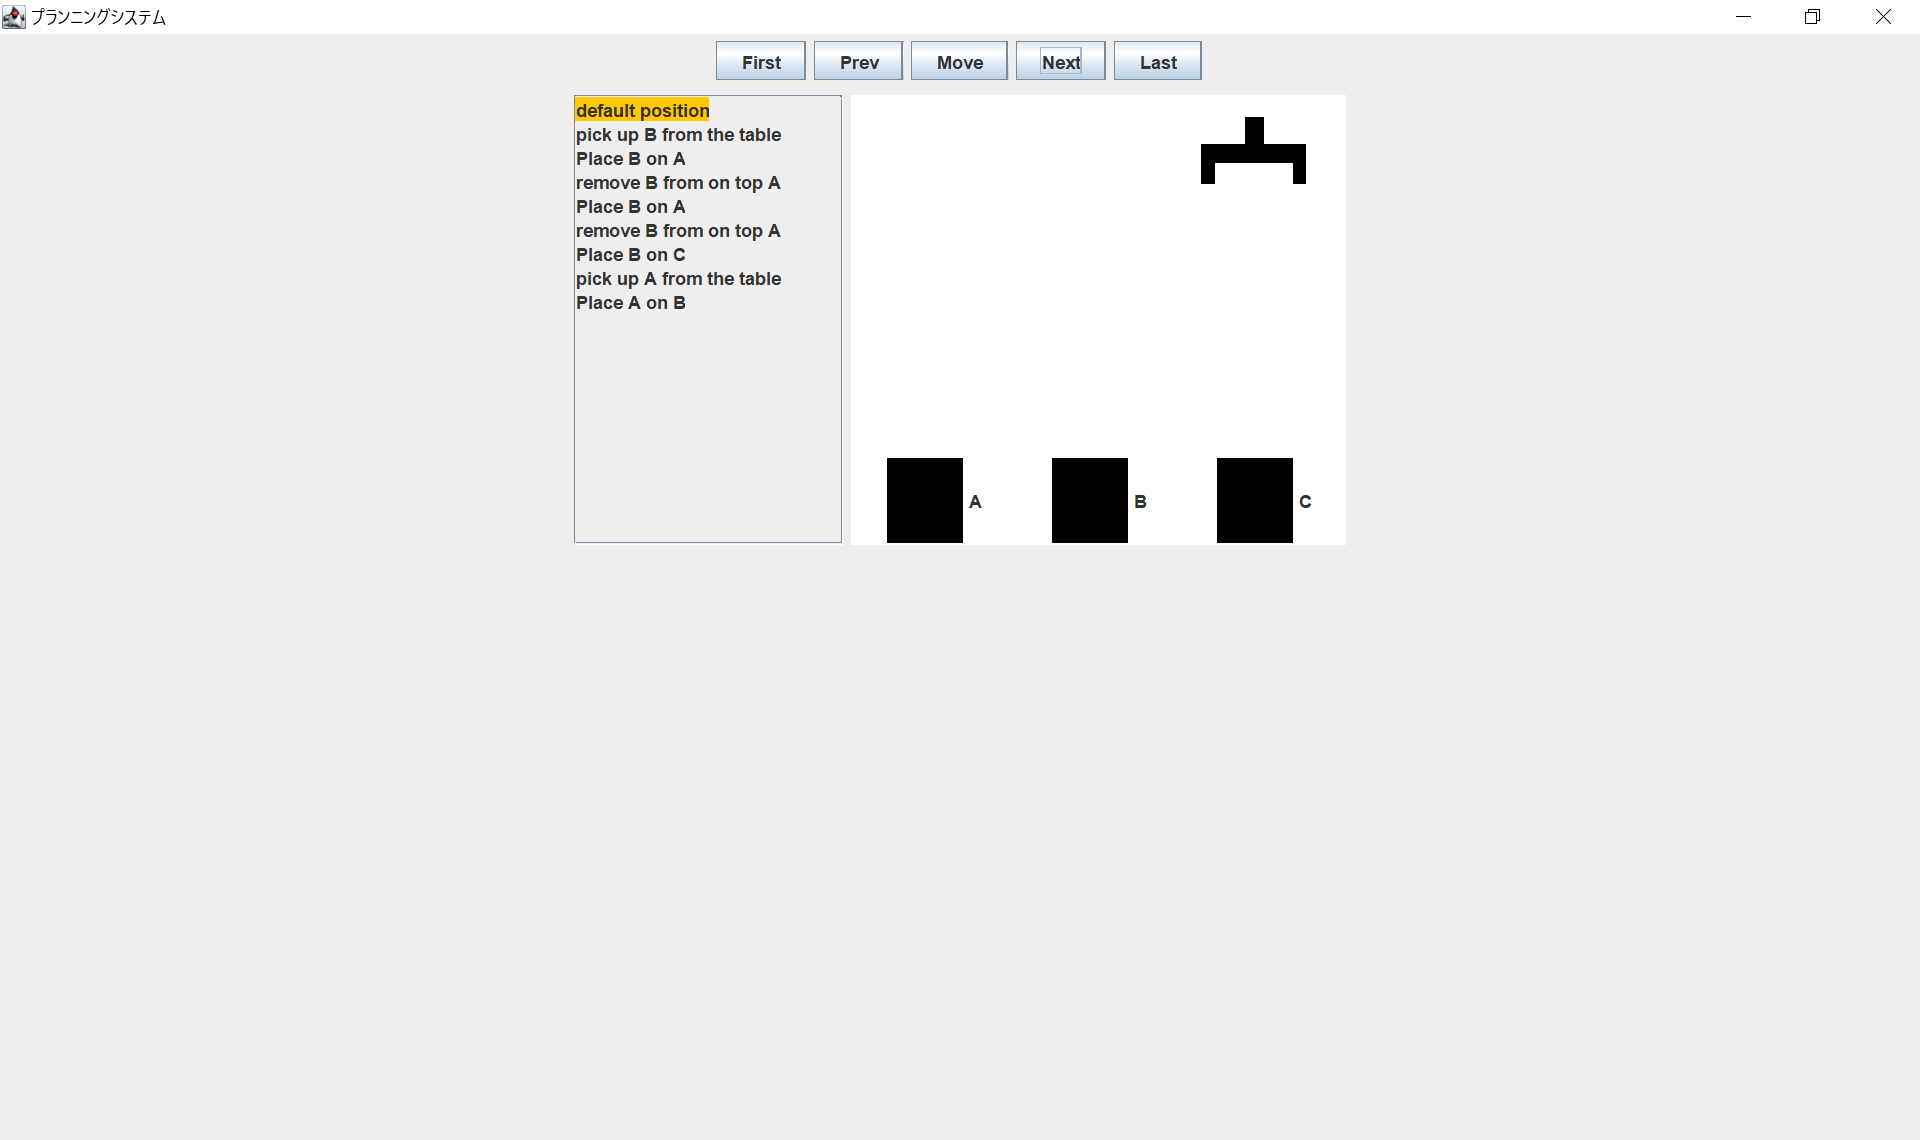
\includegraphics[scale=0.4]{images/ButOK.PNG}
    \caption{改良後のウィンドウ}
    \label{fig:ButOK}
  \end{center}
\end{figure}
ここからも分かるように,再描画後ウィンドウサイズを変更してもボタンが二重に表示されることが無くなった.\\
%\vspace{10mm}
\clearpage

次に,導出結果をより見やすくするためのMoveボタンの動作の実行結果を以下に示す.\\

実行した直後に現れる画面が以下のようになる(図\ref{fig:FirstPage}).\\

\begin{figure}[htbp]
  \begin{center}
    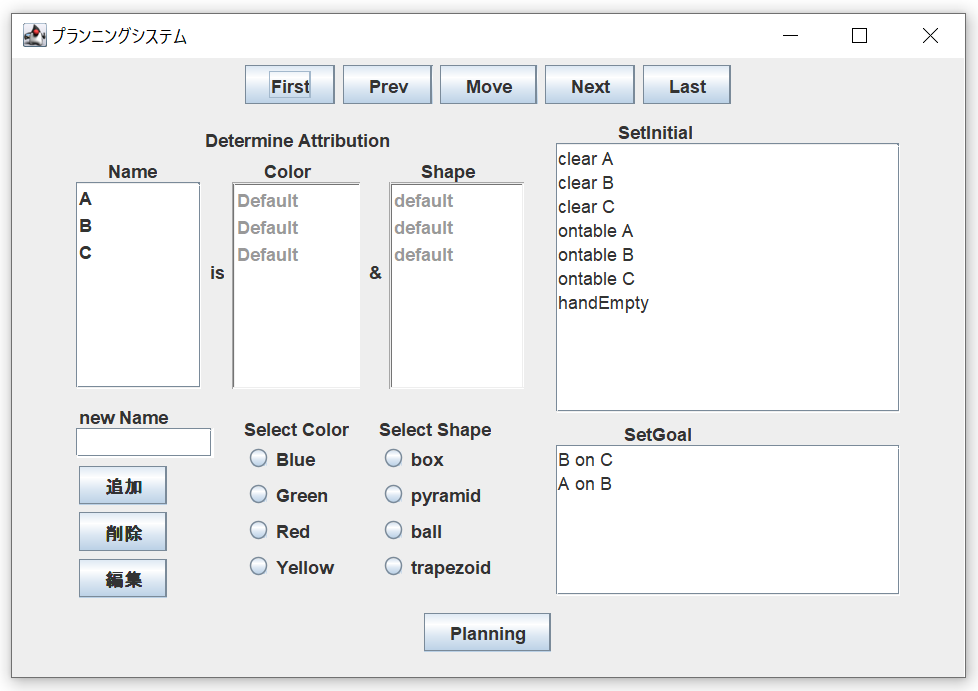
\includegraphics[scale=0.8]{images/FirstPage.PNG}
    \caption{Moveボタン追加後の初期画面}
    \label{fig:FirstPage}
  \end{center}
\end{figure}
前回の画面では,ウィンドウ上部にあるボタンが「First」「Prev」「Next」「Last」の四つであったが,今回の改良により新たに「Move」ボタンが追加されている.\\

\clearpage

Nextボタンを押すと,前回の課題同様に順に導出経路を確認することが出来る(図\ref{fig:Normal}).\\

\begin{figure}[htbp]
  \begin{center}
    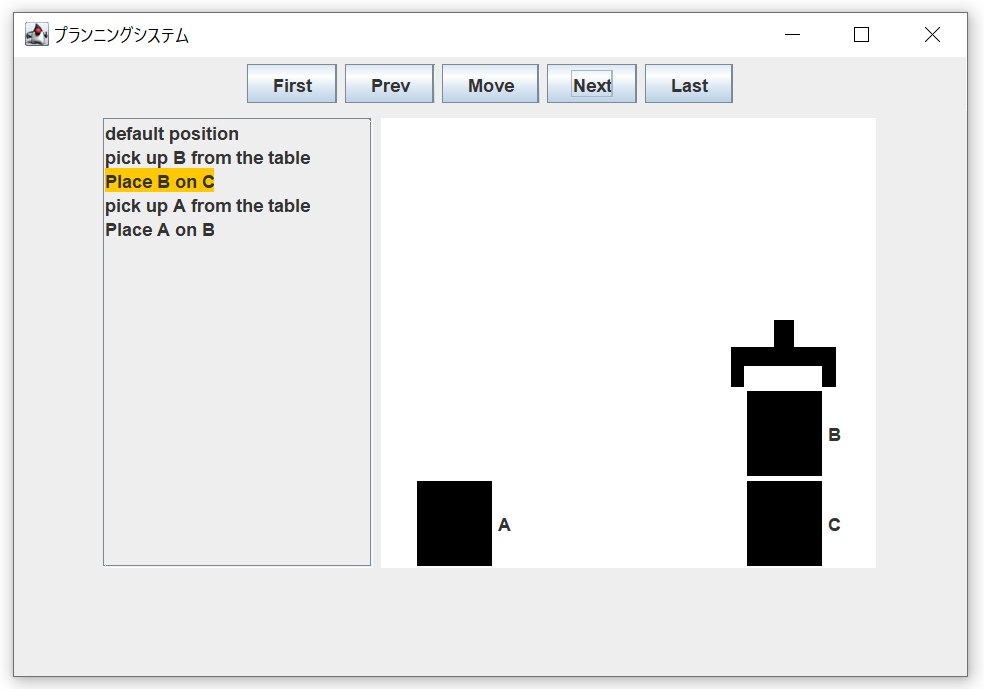
\includegraphics[scale=0.8]{images/Normal.PNG}
    \caption{Nextボタンで経路を確認するとき}
    \label{fig:Normal}
  \end{center}
\end{figure}
このとき,Nextボタンで状態が一つ進み,Prevボタンで状態が一つ戻る.またFirstボタンで初期画面に戻り,Lastボタンで最後の画面に遷移する.\par
これらの動作は前回作成したGUIと同じである.\\

\clearpage

Moveボタンを押した時の動作は以下のようになる(図\ref{fig:Move}).\\

\begin{figure}[htbp]
  \begin{center}
    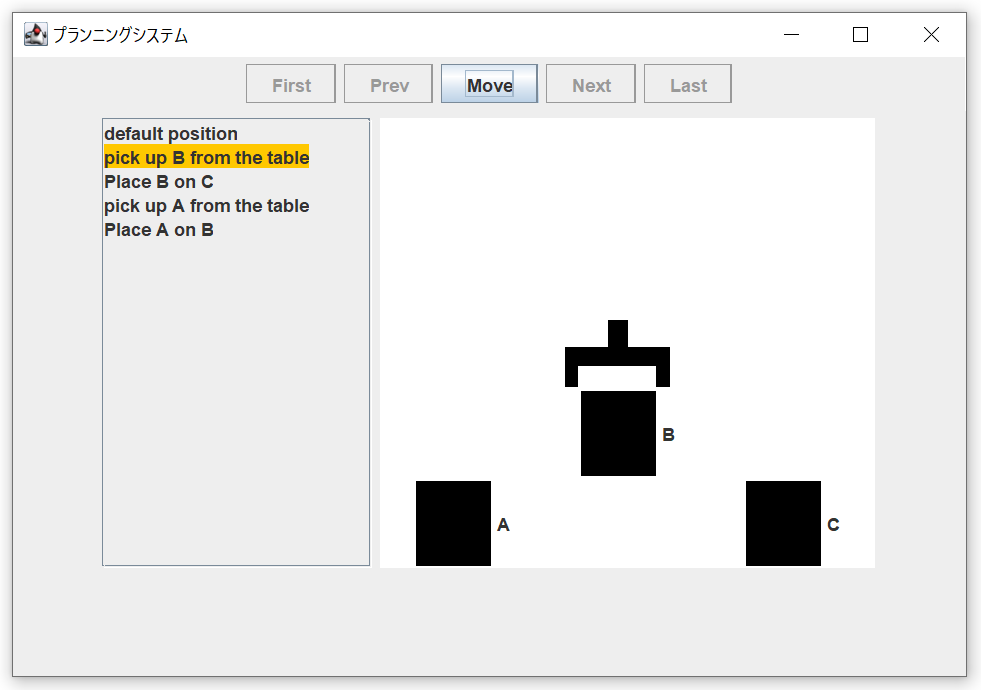
\includegraphics[scale=0.8]{images/Move.PNG}
    \caption{Nextボタンで経路を確認するとき}
    \label{fig:Move}
  \end{center}
\end{figure}
Moveボタンをクリックすると,その他のボタンが無効となり上図のようにクリック出来なくなる.さらにどの画面状態であっても初期状態の画面に遷移し,そこから一定時間ごとに導出経路が順に表示される.\par
最後に導出経路と使用したオペレータの出力画面が出力されると同時に無効になっていたボタンが有効になり,その他の操作が出来るようになる.

\clearpage
\subsection{考察}
今回の改良を行うにあたり実行結果を検証している際にGUIのウィンドウサイズを変えた際に起きてしまうバグを発見し,今回の課題としてまず改良を行った.\par
調べたところremoveAllメソッドを用いることでこの問題は解決できることが分かったが,このバグがなぜ起きるのかを調べたものの明確な答えを得ることが出来なかった.しかしこのバグが起きるのは再描画後であったため,再描画時に上書きする形で描画を行っていたことが原因ではないかと推測される.\par
前回課題ではウィンドウサイズの変更をしなくても良いGUIの作成を考えていたが,ユーザーがウィンドウサイズを変更する場合の可能性も考えてプログラムを作成する必要があると分かった.\\

さらに検証する中で,再描画時にウィンドウサイズを変更すると描画が一部消えてしまうことがあることも分かった.この場合も初めの描画時には消えることは無いため再描画に何か原因があると考えたが,これについては明確な原因とその対処方法が分からず,解決することが出来なかった.しかしマウスを近づけたりボタンをクリックすると消えた描画が元に戻るため,描画が出来ていないわけではないことは確認された.\par
この解決方法としては,再描画をしないようにプログラムを書き換える方法が考えられる.この場合私が使用しているCardLayoutでの状態遷移の描画を,再描画の際も以前のものを消さずにCardを増やす形にする方法が最も現実的であると考えた.しかしこの場合はNextボタンやPrevボタンでの処理が少し複雑になることや,繰り返しプランニングを行うことでCardの枚数が増え最終的にメモリ不足によるエラーが発生してしまうという欠点がある.そもそもGUIが再描画に適していないとも考えられたが今回の場合は描画自体は正しくできていることも考え,前回までの実装をそのまま採用した.\\

\clearpage

また以前の課題ではブロックが五つ以上ある場合は描画がGUIのウィンドウサイズを超えてしまい,ウィンドウサイズを大きくしなければ図が確認できなくなってしまうという問題があった.これを修正するため描画画面に対してスクロールバーをつけ,範囲を超えた描画を行う場合はスクロールバーを移動させ,ウィンドウサイズを変更することなく表示させることを考え実装を行った.\\

\vspace{10mm}

以下にその際のソースコードを示す(ソースコード\ref{scroll}).
\begin{lstlisting}[caption=スクロールバーの追加,label=scroll]
// 変数定義
JPanel card = new JPanel();
JPanel newpage = new JPanel();

// 画面を超えた描画時にスクロールバーにする
JScrollPane scrollpane = new JScrollPane();
// 最大描画サイズの指定
scrollpane.setPreferredSize(new Dimension(400, 350));
JViewport view = scrollpane.getViewport();
view.setView(newpage);
JPanel panel = new JPanel();
panel.add(scrollpane);
// パネルへの追加
card.add(splist);
card.add(panel);
\end{lstlisting}

この方法を用いることで,描画サイズが最大範囲を超えた時にはスクロールバーが追加されるようになった.

\clearpage

この時の実行結果が以下のようになる(図\ref{fig:tryScroll}).\\

\begin{figure}[htbp]
  \begin{center}
    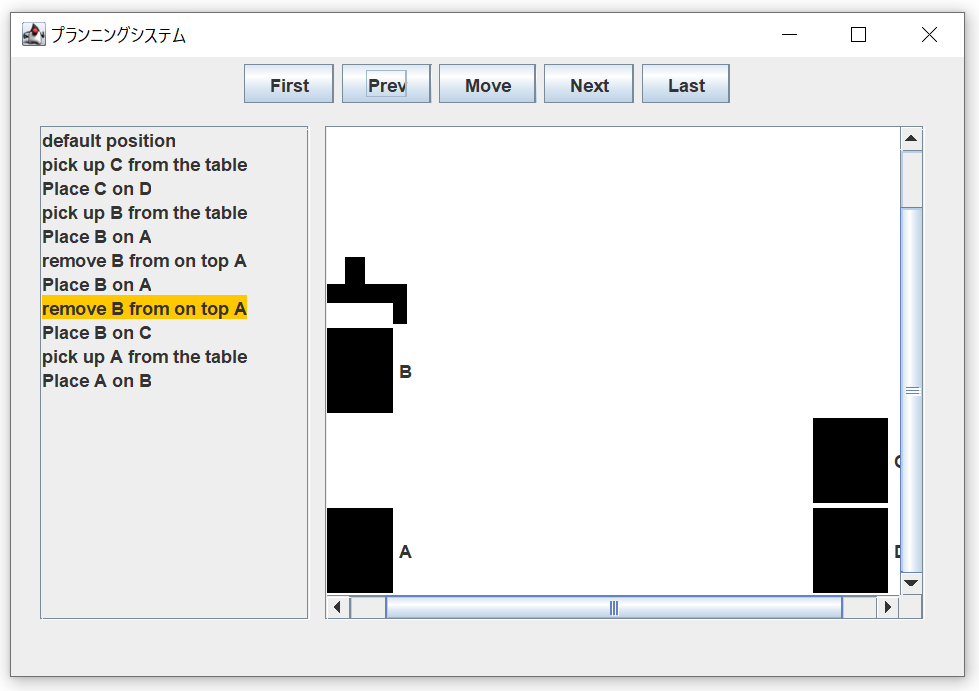
\includegraphics[scale=0.8]{images/tryScroll.PNG}
    \caption{スクロールバーを追加した場合}
    \label{fig:tryScroll}
  \end{center}
\end{figure}


ここから分かるように,スクロールバーを追加した場合描画サイズが表示可能サイズよりも大きいため,スクロールバーが出力された場合は一度にすべての状態を確認することが出来なくなってしまう.これでは現在の状態がどうなっているのか確認するのにいちいちスクロールバーを操作しなければならず,ブロックの数が増えれば増えるほど確認に大きな負担がかかる.\par
さらにスクロールバーは指定しなければ常に同じ位置にあるため,状況によってはその時動かしたブロックがスクロールバーを動かさなければ確認できない位置に存在する場合も考えられる.これではGUIとして使い難いことは明らかであるため,今回はスクロールバーの追加はしないこととした.\\

この解決方法としては,描画方法を変えることが最も効果的と考えられる.今回は描画にあらかじめ用意した画像を使用したが,この方法では表示する画像のサイズを変更することが出来ない.\par
直接描画を行う方法であればサイズの調節が可能になるため,ウィンドウサイズの変更をせず描画を行いたい場合は直接描画を行う方法が最良であると分かった.しかし前回の課題でも考察した通りその方法では座標設定を全て自身で行わなければならないため,座標管理が複雑になってしまうだけでなく,GUIの良さであるレイアウトマネージャーを活用出来なくなってしまう.このことから今回もこの方法での実装は行わないこととした.\\

\vspace{10mm}

Moveボタンの追加に関しては,動画のように滑らかな動きで経路を表現したいと考えたが,調べたところ滑らかな動きを実現するためにはレイアウトマネージャーを使用せずに座標で管理を行わなければならないことが分かった.前述の理由などから前回課題で作成したプログラムを活用して改良することを考え,今回は滑らかな動きをせず経路の過程を一回の操作(ボタンのクリック)で確認できるようにすることを目標とした.\\

導出経路の過程を表示するために用いたのがCardLayoutであったため,これを一定時間ごと次の画面に遷移させることで過程の表示が動的に行えると考えた.どの状態にあってもMoveボタンをクリックすれば初期状態から目標状態までの過程を表示できるようにするため,Moveボタンをクリックした段階でまず初期状態の画面に遷移し,そこから導出されている経路のCard枚数分だけ次のページへの遷移を繰り返す形とした.\par
このとき実行結果で述べたとおり他のボタンを動かせる状態にしておくと,Moveボタンによる繰り返しの回数と遷移状態がずれてしまうため表示がずれてしまう.そのため,Moveボタンで動作が行われている際はその他のボタンは無効にすることで正しい動作が行えるようにした.\\

%\vspace{10mm}

またこの機能を実装する中で,ボタンの操作検出による動作中は繰り返し作業や更なるボタンの操作を行うことが出来ないことが分かった.試行錯誤の中で,前回まではボタンのクリック操作をActionEventで検知していたが,MouseEventのmousePressedメソッドを用いればこれらの問題を解決できるのではないかと考え,mousePressedメソッドを使った実装を行った(ソースコード\ref{timer}参照).結果的にはMouseEventでも上記の動作は行うことが出来なかったため,その他の方法を調べ,タイマークラスを用いる方法を実装して求めている動作を実現させた.\par
結果的にはタイマークラスを用いることでMouseEventのmousePressedメソッドでなくActionEventでの実装でも同様の結果が得られることが分かったが,今回は様々な実装方法を学ぶという面からMouseEventを用いてプログラムを作成した.\par
GUIの場合も,同じ機能であっても様々な方法を用いて実装を行えることが分かった.

\section{感想}
今回は前回の課題に改良を加えるため,基本的な方針としては前回作成したGUIの機能でより良くしたいと感じた部分を修正した.その際に作成者では分からないユーザーの使い難さがあると考え,友人に作成したGUIを見せ,どのような部分に改良が必要かの意見を出してもらった.その中で出た改善案の中から自分にも実装出来そうなものを作成した.実際に自分以外の人にGUIを見てもらうことで,自身では気づけなかったGUIの使い難さを知ることが出来た.中には私は使い難いと感じていなかった機能が実はもっと使い易くできると分かった部分もあり,今回の課題は使用者のことを考えたGUI作成の難しさを改めて考えさせられるものであった.\\

また,ユーザーがどのような操作をするかは分からないため,出来る限り様々な可能性を考えそれぞれに対応した動作が出来るプログラムを作成することの大切さを難しさを感じた.\par
そのため,他の班の人がどのようなGUIをどのように作成したのかを見て自分の学びにつなげたいと強く感じた.

% 参考文献
\begin{thebibliography}{99}
\bibitem{Java新} 新谷虎松『Javaによる知能プログラミング入門』コロナ社,2002年.
\bibitem{Swing} Let'sプログラミング Swingを使ってみよう, \url{https://www.javadrive.jp/tutorial/} (2019年1月3日アクセス).
\end{thebibliography}
\end{document}
